\section{Relacje binarne}

\begin{table}[h]
    \centering
    \begin{tabular}{|c|c|c|c|}
    \hline
    $R_2$ & a & b & c \\ \hline
    a & 1 & 1 & 0 \\ \hline
    b & 0 & 0 & 0 \\ \hline
    c & 0 & 0 & 0 \\ \hline
    \end{tabular}
\end{table}

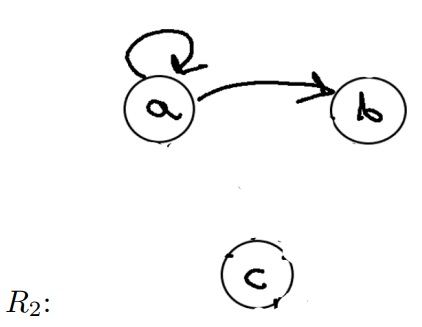
\includegraphics[scale=0.5]{img/grafR2.png}

\subsection{Własności relacji}

Niech dana będzie relacja binarna na $ R \subseteq X \times X $

Za przykładowe uniwersum posłuży nam zbiór $U = \{ a, b, c, d \} $ \\

Własności relacji i ich warunki

\begin{itemize}
    \item Zwrotna -- $\forall x \in X (<x,x> \in R)$
    
    Aby było zwrotna w relacji \textbf{musi} znaleźć się $ \{ <a, a>, <b, b>, <c, c>, <d, d> \} $

    \item Przeciwsymetryczna -- $\forall x \in X(\neg <x, x> \in R) $
    
    Aby była przeciwzwrotna to w relacji \textbf{nie może} znaleźć się \textbf{żadna} z tych par \linebreak 
    $ <a, a>, <b,b>, <c,c>, <d,d> $
    
    \item Symetryczna -- $ \forall x, y \in X(<x,y> \in R \Rightarrow <y,x> \in R) $
    
    Aby była symetryczna to \textbf{każda istniejąca para w relacji} musi mieć swoje lustrzane odbicie. Na przykład:
    $ \{ <a,b>, <b,a>, <a, a>, <b,c>, <c,b> \} $

    \item Asymetryczna -- $\forall x,y \in X((<x,y> \in R \land (y,x) \in R) \Rightarrow x=y) $
    
    \item Przeciwsymetryczna -- $\forall x,y \in X(<x,y> \in R) \Rightarrow \neg <y,x> \in R) $
\end{itemize}